\documentclass[10pt, letterpaper]{article}

\usepackage{preamble}

\begin{document}

\begin{multicols}{2}
        \textbf{\fontsize{24 pt}{24 pt}\selectfont David López del Pino}

        \vspace{0.4 cm}

        \normalsize

        \hspace{0.4 mm}\mbox{{\color{black}\footnotesize\faMapMarker*}\hspace*{0.16 cm}Málaga, Spain}%

        \mbox{\hrefWithoutArrow{mailto:lopezdelpinodavid@gmail.com}{\color{black}{\footnotesize\faEnvelope[regular]}\hspace*{0.13cm}lopezdelpinodavid@gmail.com}}%

        \mbox{\hrefWithoutArrow{tel:+34-622-23-23-87}{\color{black}{\footnotesize\faPhone*}\hspace*{0.13cm}622 23 23 87}}%

        % \mbox{\hrefWithoutArrow{https://yourwebsite.com/}{\color{black}{\footnotesize\faLink}\hspace*{0.13cm}yourwebsite.com}}%
        % \kern 0.25 cm%
        % \AND%
        % \kern 0.25 cm%
        \mbox{\hrefWithoutArrow{https://linkedin.com/in/david-lopez-del-pino}{\color{black}{\footnotesize\faLinkedinIn}\hspace*{0.13cm}david-lopez-del-pino}}%

        \mbox{\hrefWithoutArrow{https://github.com/dldelpino}{\color{black}{\footnotesize\faGithub}\hspace*{0.13cm}dldelpino}}%

        \vfill\null
        \columnbreak

        \begin{flushright}
            \begin{tikzpicture}
                \node [inner sep=0pt,,outer sep=0pt,clip,rounded corners=0.5cm] (pict) at (0,0) {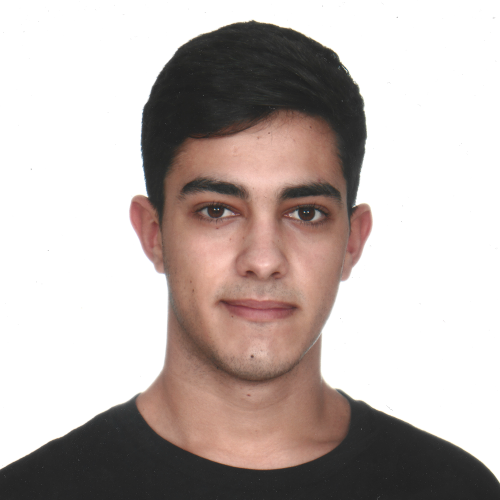
\includegraphics[width = 3.5cm]{img.png}};
                \node[draw=gray,line width = 1.2pt,fit=(pict),rounded corners=.55cm,inner sep=0pt]    {};
            \end{tikzpicture}
        \end{flushright}
\end{multicols}

    \section{About me}
        \begin{onecolentry}
            Recent graduate in Mathematics with solid knowledge in Python development, data analysis and problem solving. I am looking to join a team where I can gain experience and develop my professional career.

            \vspace{0.2 cm}

            I consider myself an energetic, determined and responsible person, with great learning capacity and good time management and communication skills. I have a proactive attitude towards acquiring new knowledge and I am motivated to improve my skills and face new challenges.

        \end{onecolentry}

    \section{Education}

        \begin{twocolentry}{
            
        \textit{September 2021 – July 2025}}
            \textbf{University of Málaga}

            \textit{Bachelor of Mathematics}
        \end{twocolentry}

        \vspace{0.10 cm}
        \begin{onecolentry}
            \begin{highlights}
                \item \emph{Average grade:} 8.94/10 % (\href{https://example.com}{a link to somewhere})
                \item \emph{Bachelor Thesis:} Results on convergence of Fourier series
                \item Distinction in 11 subjects
            \end{highlights}
        \end{onecolentry}
    
    \section{Technical skills}
 
        \begin{twocolentry}{
            
        \textit{2022 – 2025}}
            \textbf{Programming in Python}

            \textit{University of Málaga}
        \end{twocolentry}

        \vspace{0.10 cm}
        \begin{onecolentry}
            \begin{highlights}
                \item Numerical resolution of partial differential equations using the finite difference method and the finite element method.
                \item Visualisation of solutions of differential equations and precision analysis with NumPy, SciPy and Matplotlib.
                \item Extracting data from web pages using BeautifulSoup.
                \item Analysis and manipulation of data and tabular structures using Pandas.
            \end{highlights}
        \end{onecolentry}

    \section{Technologies}

        \begin{onecolentry}
            \textbf{Programming languages:} Python, Scala, Haskell, C++, C\#, Java, JavaScript, SQL
        \end{onecolentry}

        \vspace{0.2 cm}

        \begin{onecolentry}
            \textbf{Other technologies:} HTML, CSS, React, LaTeX, Wolfram Mathematica, Git, Microsoft Office, MySQL
        \end{onecolentry}

    \section{Languages}

        \begin{twocolentry}{
            
        \textit{September 2023}}
            \textbf{English (C2)}

            \textit{Cambridge English: Advanced}
        \end{twocolentry}

        \vspace{0.10 cm}
        \begin{onecolentry}
            \begin{highlights}
                \item \emph{Score:} 204/210 % (\href{https://example.com}{a link to somewhere})
            \end{highlights}
        \end{onecolentry}

        \vspace{0.2 cm}
    
        \begin{twocolentry}{
            
        \textit{April 2021}}
            \textbf{French (B2)}

            \textit{Diplôme d'Études en Langue Française (DELF)}
        \end{twocolentry}

        \vspace{0.10 cm}
        \begin{onecolentry}
            \begin{highlights}
                \item \emph{Score:} 87.5/100 % (\href{https://example.com}{a link to somewhere})
            \end{highlights}
        \end{onecolentry}

        \vspace{0.2 cm}

        \begin{onecolentry}
            \textbf{Spanish (mother tongue)}
        \end{onecolentry}

\end{document}